\chapter{Imaging Heterogeneity: State of the
Art}\label{imaging-heterogeneity-state-of-the-art}\label{ch:4}

This chapter reviews how imaging heterogeneity has been approached, from
qualitative visual assessment through radiomics to habitat imaging. The
goal is to establish the scientific context for the work in this thesis
and to identify the methodological gaps that motivate it. This chapter
largely follows the comprehensive reviews carried out by O'Connor (J. P.
O'Connor et al., 2008; J. P. B. O'Connor et al., 2015; O'Connor, 2017).

\section{Definition and Historical Context}\label{definition-and-historical-context}

At the macroscopic scale of radiology, intratumor heterogeneity refers
to variations in imaging phenotype observed within tumor . These are
differences in intensity, texture, enhancement patterns, and spatial
organization that may reflect underlying biological variation. In the
literature, the term has been used inconsistently. Different authors
have referred to imaging heterogeneity when describing abstract
radiological phenotypes linked to CT density, global texture features
computed across whole tumors, or subregions (i.e. habitats). In this
thesis, we focus on the latter. We define imaging heterogeneity as the
spatial variation in tissue composition that can be detected and
quantified from imaging and that corresponds to known histopathological
structures such as viable tumor, necrosis, and fibrosis.

What the literature agrees on is twofold. First, clinical imaging is
currently underutilized. We extract only a fraction of the information
contained in routine scans, primarily size, location, and number of
lesions. Second, tumor heterogeneity is clinically important.
Heterogeneity is thought to drive treatment resistance and tumor
adaptation. In the era of precision medicine, where patients receive
targeted therapies requiring monitoring, non-invasive assessment of
spatial and temporal heterogeneity could inform treatment decisions.

Approaches to quantifying imaging heterogeneity have evolved over time
(\Cref{fig:4.1}).The idea of using computers to
extract quantitative information from medical images dates back to the
1960s, when Lodwick first applied computational analysis to chest
radiographs and introduced the concept of computer-aided diagnosis
\citep{lodwickCodingRoentgenImages1963}. A decade later, Haralick developed the
gray-level co-occurrence matrix (GLCM), establishing the mathematical
foundation for texture analysis that would later support radiomics
\citep{haralickTexturalFeaturesImage1973}. Early applications of clustering to identify
tumor subregions appeared in the 2000s \citep{caranoQuantificationTumorTissue2004}, predating
the formal concept of habitat imaging. Around the same time,
quantitative approaches to response assessment emerged, including the
Choi criteria incorporating CT attenuation changes \citep{choiCorrelationComputedTomography2007}
and morphological response criteria for colorectal liver metastases
\citep{chunAssociationComputedTomography2009}.

The field was formalized in the early 2010s. The term radiomics was
coined in a seminal paper of 2012 \citep{lambinRadiomicsExtractingMore2012}, rebranding
texture analysis as a systematic, high-throughput approach to extracting
quantifiable data from medical images. A year later, the concept of
imaging habitats was introduced \citep{gatenbyQuantitativeImagingCancer2013}. The landmark
study by Aerts and colleagues \citep{aertsDecodingTumourPhenotype2014} demonstrated that
radiomic features could predict clinical outcomes across multiple cancer
types, catalyzing widespread interest in the field. Standardization
followed with PyRadiomics \citep{vangriethuysenComputationalRadiomicsSystem2017} and the Image
Biomarker Standardization Initiative (IBSI) \citep{zwanenburgImageBiomarkerStandardization2020}.

\begin{figure}[htbp]
\centering
\includegraphics[width=0.95\textwidth]{fig_4_1.pdf}
\caption[Evolution of approaches to imaging heterogeneity]{\textbf{Evolution of approaches to imaging heterogeneity.}
Timeline illustrating the methodological progression in quantifying
tumor heterogeneity from medical images. Early foundations include
computer-aided diagnosis \citep{lodwickCodingRoentgenImages1963} and texture analysis
mathematics \citep{haralickTexturalFeaturesImage1973}. The 2000s saw early subregion
analysis \citep{caranoQuantificationTumorTissue2004} and quantitative response criteria (Choi
et al., 2007; Chun, 2009). The field was formalized in the early 2010s
with the definition of radiomics \citep{lambinRadiomicsExtractingMore2012} and habitats
\citep{gatenbyQuantitativeImagingCancer2013}, followed by the demonstration of prognostic
value across cancers \citep{aertsDecodingTumourPhenotype2014} and standardization
initiatives \citep{vangriethuysenComputationalRadiomicsSystem2017,zwanenburgImageBiomarkerStandardization2020}. The
late 2010s marked the entry of deep learning into radiology (Lakhani \&
Sundaram, 2017) and foundation models for cancer imaging biomarkers have
emerged most recently \citep{paiFoundationModelCancer2024}. The trajectory shows a shift
from qualitative assessment and handcrafted features toward learned
representations. Created with Biorender.com.}
\label{fig:4.1}
\end{figure}

More recently, deep learning approaches have begun to complement or
replace handcrafted features. Lakhani and Sundaram (2017) demonstrated
the application of deep convolutional neural networks to chest
radiograph interpretation, marking the entry of deep learning into
mainstream radiology research \citep{lakhaniDeepLearningChest2017}. Foundation
models are now emerging in medical imaging, including models
specifically designed for cancer imaging biomarker discovery (Pai et
al., 2024). These developments represent a shift from handcrafted
features designed by humans to learned representations discovered by
neural networks.

\section{Qualitative and Conventional Quantitative Approaches}\label{qualitative-and-conventional-quantitative-approaches}

The simplest approach to imaging heterogeneity is qualitative visual
assessment, the subjective evaluation of tumor characteristics by
radiologists without explicit measurement. These are the classic
features noted in radiology reports: morphology, enhancement patterns,
and relationship with surrounding tissues. A radiologist might describe
margins as irregular versus well-defined, enhancement as homogeneous
versus heterogeneous, or note the presence of rim enhancement.

For colorectal liver metastases specifically, qualitative morphological
criteria were proposed to improve response assessment \citep{chunAssociationComputedTomography2009}. The
authors based the criteria on overall attenuation (heterogeneous, mixed,
or homogeneous), tumor-liver interface (ill-defined, variable, or
sharp), and peripheral rim of enhancement (present or absent). They
observed that metastases treated with anti-angiogenic therapy often
transform from heterogeneous, irregular lesions with ill-defined borders
into homogeneous, hypoattenuating lesions with well-defined borders.
Importantly, morphologic response. \Cref{fig:4.2}
shows an example of pre- and post-treatment CT{} scans of two patients
response.

\begin{figure}[htbp]
\centering
\includegraphics[width=0.8\textwidth]{fig_4_2.png}
\caption[Example of qualitative approach to imaging heterogeneity]{\textbf{Example of qualitative approach to imaging heterogeneity.}
Pre- and posttreatment CT scans showing RECIST stable disease and
morphological optimal response (top) and incomplete response (bottom).
Optimal response is characterized by homogenous attenuation and sharp
tumor-liver interface while incomplete response is characterized.
Adapted from Chun, 2009.}
\label{fig:4.2}
\end{figure}

Conventional quantitative approaches use objective numerical values
derived from standard imaging. The most direct quantitative measure from
CT{} is the Hounsfield unit value itself. In CECT, the
difference in HU between pre-contrast and post-contrast images reflects
contrast agent accumulation, which is related to tissue vascularity.
Studies have shown that changes in tumor attenuation can detect early
anti-vascular effects of bevacizumab before size changes occur
\citep{koukourakisEarlyAntivascularEffects2007}. A seminal study in this area is the work of
Choi et al., 2007, who extended RECIST by incorporating HU changes for
gastrointestinal stromal tumors (GIST) treated with imatinib, a targeted
therapy. Similar to the therapies discussed in Section
\Cref{treatment-landscape-and-selection-challenges}, imatinib is a cytostatic drug,
inhibiting growth and division of cancer cells rather than killing them
outright. In the study, a 15\% reduction in HU on CECT
was included alongside size criteria, acknowledging that for targeted
therapies, compositional changes captured by attenuation matter. The use
of Choi criteria has been suggested for metastatic colorectal cancer,
but current evidence is insufficient to recommend them routinely
\citep{zamboniESREssentialsResponse2024}.

However, these approaches have limitations. First, both approaches
provide single-point measurements or global descriptions that fail to
capture spatial complexity within tumors. Second, qualitative assessment
suffers from inter-observer variability and HU values are sensitive to
acquisition parameters (tube voltage, reconstruction kernel, contrast
timing). For an imaging measurement to serve as a biomarker, it must be
quantifiable and reproducible (J. P. B. O'Connor et al., 2017). The
qualitative observations and conventional quantitative measures
described above showed that imaging heterogeneity contains prognostic
information, but they lacked the standardization required for clinical
use. The field needed a systematic effort to convert these observations
into proper quantitative imaging biomarkers with demonstrated
reproducibility. This came in the 2010s with the formalization of
radiomics.



\section{Radiomics}\label{radiomics}

The idea of extracting quantitative features from medical images is not
new. Historically, this work was known as texture analysis and included
different methods for quantifying spatial patterns in images. The most
widely used was the gray-level co-occurrence matrix (GLCM) (Haralick et
al., 1973), which counts how often specific pairs of intensity values
appear next to each other in an image. Texture analysis was applied to
medical imaging throughout the 1990s and 2000s. Early studies
demonstrated that CT texture features could predict survival in
colorectal cancer \citep{milesColorectalCancerTexture2009}, decode gene expression patterns
in hepatocellular carcinoma \citep{segalDecodingGlobalGene2007}, and correlate with
histopathological characteristics in non-small cell lung cancer (Kawata
et al., 2012).

What changed in the 2010s was not the underlying mathematics but the
framing and infrastructure. The term \emph{radiomics} was coined by
Lambin and colleagues \citep{lambinRadiomicsExtractingMore2012}, rebranding texture analysis
as a systematic, high-throughput approach to extracting quantifiable
data from medical images. The real catalyst for widespread adoption was
PyRadiomics \citep{vangriethuysenComputationalRadiomicsSystem2017}, an open-source and
user-friendly Python package that standardized the computation of
handcrafted radiomic features. An additional effort to push radiomic
features towards clinical biomarkers was the Image Biomarker
Standardization Initiative (IBSI) \citep{zwanenburgImageBiomarkerStandardization2020}. The IBSI
established consensus definitions for feature computation, addressing
the problem that different groups had previously implemented features
differently, making comparison across studies difficult.

While radiomic features are broadly defined as any quantitative measures
derived from radiological images, the term is most commonly used in the
literature to denote \emph{handcrafted} radiomic features (a convention
largely shaped by the influence of PyRadiomics). Handcrafted features
are derived from explicitly defined mathematical formulas or matrices
designed by humans, such as the GLCM (\Cref{fig:4.3}). They are typically grouped into three categories: shape features
that describe tumor geometry (e.g., volume, surface area, sphericity),
first-order features that summarize the distribution of voxel
intensities (e.g., mean, variance, skewness), and texture features that
quantify spatial relationships between voxels (e.g., entropy, contrast,
homogeneity derived from GLCM and similar matrices).

The defining characteristic of handcrafted features is that they are
designed a priori, based on domain knowledge, before observing the data.
This is also their main limitation: their usefulness depends on whether
the predefined features capture the patterns that are relevant for a
given task. Traditional machine learning methods cannot adapt the
feature representation itself \citep{goodfellowDeepLearning2016}: when applied
directly to raw pixel data without carefully engineered inputs, they
tend to perform poorly. Deep learning \citep{lecunDeepLearning2015} overcomes
this limitation by learning hierarchical feature representations
directly from data, progressively building complex concepts from simpler
ones across multiple layers. Rather than requiring humans to specify
which image patterns matter, deep neural networks learn representations
optimized for the task at hand. More recently, foundation models
\citep{bommasaniOpportunitiesRisksFoundation2021} have emerged as a further development: large
neural networks pretrained on vast datasets that learn general-purpose
representations and can be adapted to specific tasks with minimal
additional training. In the context of this thesis, which began in 2021,
deep learning and foundation model approaches for radiomics were not yet
sufficiently mature. The methods developed here therefore focus on
handcrafted features, although comparisons with deep learning--based
embeddings are presented in Chapter~\ref{ch:7}.

A relevant distinction in radiomics is how features are computed
spatially (\Cref{fig:4.3}). Computing features over
the entire tumor, producing a single value per feature, is known as
region-of-interest-wise (ROI-wise) or standard radiomics. This is the
dominant approach because most radiomics studies use supervised
learning, which requires fixed-length feature vectors as input.
Voxelwise radiomics computes features locally, within a sliding kernel
centred on each voxel. For example, to compute voxelwise GLCM entropy,
the algorithm defines a neighbourhood around each voxel, computes
entropy within that neighbourhood, and assigns the result to the central
voxel. This produces a feature map rather than a single number,
preserving where heterogeneity is located within the tumor. The standard
radiomics pipeline is straightforward: extract features from segmented
tumors, select or reduce features to avoid overfitting, and train a
supervised model to predict a clinical endpoint.

\begin{figure}[htbp]
\centering
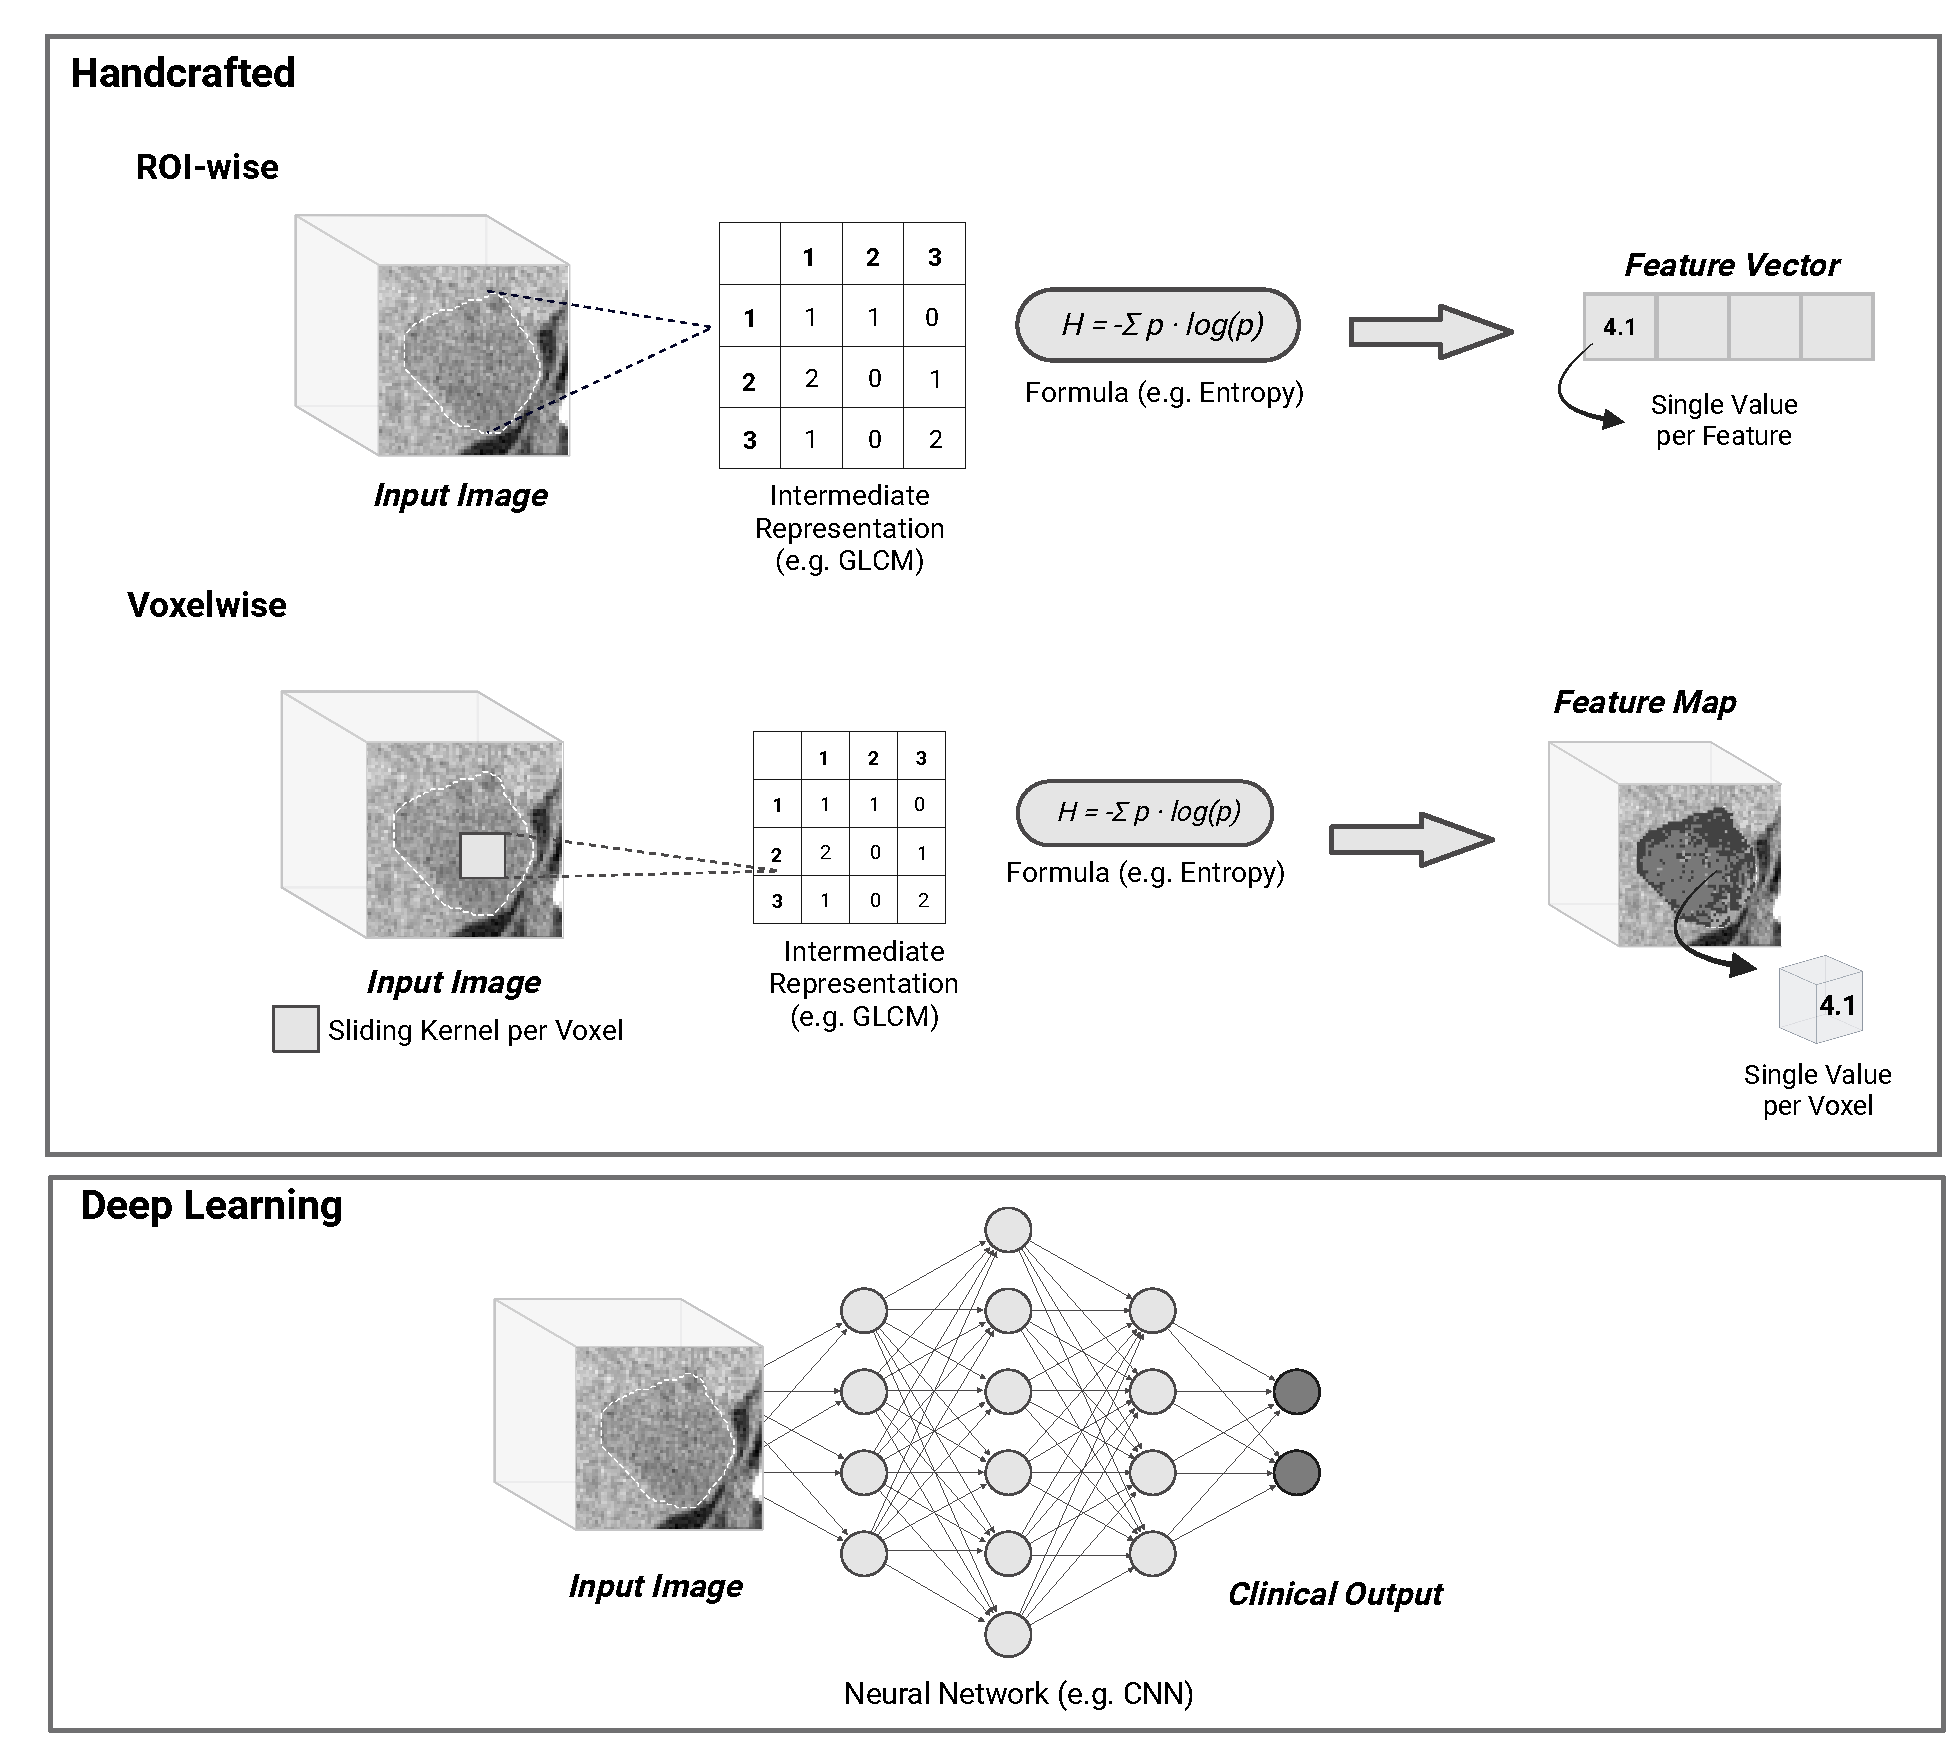
\includegraphics[width=0.95\textwidth]{fig_4_3.pdf}
\caption[Schematic comparison of radiomics feature extraction methods]{\textbf{Schematic comparison of radiomics feature extraction methods.}
Handcrafted Radiomics: Features are derived from explicit intermediate
mathematical representations, such as the Gray-Level Co-occurrence
Matrix (GLCM). In the ROI-wise approach (top), a single large GLCM is
accumulated over the entire tumor mask, and a formula (e.g., for
entropy) is applied once to yield a single global value. In the
Voxelwise approach (bottom), a small, local GLCM is computed within a
sliding kernel around each voxel. The formula is applied to this local
matrix, and the resulting value is assigned to the center voxel,
generating a spatial feature map. Deep Learning: The raw input image is
passed directly through a neural network (e.g., a CNN) to learn
abstract, hierarchical feature representations (embeddings) optimized
for a specific task, without explicit human-defined formulas or
intermediate matrix representations. Created with BioRender.com.}
\label{fig:4.3}
\end{figure}

The limitation of ROI-wise radiomics is that it implicitly assumes
tumors are sufficiently homogeneous that averaging captures their
essential properties. As discussed in Chapter~\ref{ch:3}, colorectal liver
metastases are histologically heterogeneous, with viable tumor,
necrosis, and fibrosis distributed in spatial patterns. Averaging over
this heterogeneity may discard clinically relevant information.



\section{Habitat Imaging}\label{habitat-imaging}

The idea of partitioning tumors into spatially distinct subregions based on imaging characteristics predates the term \emph{habitat}. In the 2000s and early 2010s, several studies already proposed the use of clustering algorithms to study intratumor heterogeneity (mainly necrosis and viable tumor) for several cancer types in preclinical models \citep{caranoQuantificationTumorTissue2004,divinePopulationBasedGaussianMixture2016,henningMultispectralQuantificationTissue2007} using PET and MRI imaging modalities.

The term habitat and its ecological framing were introduced in 2013
\citep{gatenbyQuantitativeImagingCancer2013}. Drawing on landscape ecology, they proposed that
tumors could be understood as ecosystems containing distinct habitats
with different environmental conditions. Just as a forest contains
distinct microenvironments with different species compositions, a tumor
contains regions with different blood flow, oxygenation, and cellular
populations. According to the authors, the heterogeneous environment may
drive tumor evolution (e.g., hypoxic habitats select for cells with
aggressive, therapy-resistant phenotypes) and therefore habitats might
be worth studying. This ecological framing was subsequently applied to
breast cancer DCE-MRI by the same group \citep{chaudhuryIdentifyingMetastaticBreast2015},
establishing the conceptual foundation for the field. The field remained
relatively small throughout the 2010s, with most radiomics research
focusing on supervised learning approaches that required whole-tumor
feature vectors.

To date, most habitat imaging studies have used MRI rather than CT.
This is mainly due to the richer biological information available from
multiparametric MRI: diffusion-weighted imaging provides the apparent
diffusion coefficient (ADC), which correlates with cellularity; dynamic
contrast-enhanced sequences yield perfusion parameters such as Ktrans
and ve; and T2-weighted imaging reflects tissue water content and edema.
These parameters have known relationships to tissue biology, making
habitat interpretation more straightforward.

This advantage was first demonstrated in glioblastoma, where Katiyar and
colleagues \citep{katiyarNovelUnsupervisedSegmentation2017} applied spatially regularised spectral
clustering to mpMRI in mouse xenografts, achieving strong
correlation with histological tissue fractions of necrosis and viable
tumor. This was later shown in breast cancer mouse models
\citep{jardim-perassiMultiparametricMRICoregistered2019}, where habitats derived from six MRI
parameters were validated against co-registered histology using
3D-printed tumor moulds (\Cref{fig:4.4}). The
resulting habitats corresponded to viable-normoxic, viable-hypoxic,
nonviable-hypoxic, and nonviable-normoxic tissue types, validated
against H\&E staining, pimonidazole (a hypoxia marker), and CD31 (a
vasculature marker). Beyond biological validation, imaging habitats have
been shown to correlate with clinical outcomes, mainly in glioblastoma
\citep{waqarVisualisingSpatialHeterogeneity2022}. The most prominent study computed vascular
habitats from perfusion MRI and demonstrated that they were highly
prognostic at presurgery \citep{juan-albarracinGlioblastomaVascularHabitats2018}.

\begin{figure}[htbp]
\centering
\includegraphics[width=0.95\textwidth]{fig_4_4.png}
\caption[Examples of MRI-based habitat imaging]{\textbf{Examples of MRI-based habitat imaging.}
\textbf{(A)} Preclinical breast cancer model illustrating biological
validation of imaging habitats. Habitats were defined by clustering six
MRI parameters (T2, T2*, ADC, and DCE kinetic metrics) using a Gaussian
Mixture Model. The resulting spatial maps (bottom center) were validated
against co-registered histology (right), where habitats correlated with
specific biological microenvironments: viable-normoxic (green),
viable-hypoxic (magenta/yellow), and nonviable/necrotic (blue) regions,
confirmed by H\&E, pimonidazole (hypoxia), and CD31 (vasculature)
staining. Adapted from Jardim-Perassi et al., 2019. \textbf{(B)}
Glioblastoma illustrating vascular habitats derived from perfusion MRI.
Tumors are partitioned into four distinct vascular habitats based on
perfusion characteristics: High Angiogenic Tumor (HAT, red), Low
Angiogenic Tumor (LAT, yellow), Infiltrated Peripheral Edema (IPE,
green), and Vasogenic Peripheral Edema (VPE, blue). These habitats have
been shown to differ in survival prognosis. Adapted from
Juan-Albarracín et al., 2018.}
\label{fig:4.4}
\end{figure}

CT-based habitat imaging has received less attention across all tumor
types, likely because CT provides fewer biologically interpretable
parameters. CECT reflects vascularity, and Hounsfield
units correlate broadly with tissue density, but the relationship
between CT intensity and specific tissue types is less direct than for
MRI-derived parameters.

Two studies have applied habitat imaging to colorectal liver metastases,
both using MRI rather than CT as well. In one study, researchers used
a semi-automated clustering approach based on PCA of DCE-MRI contrast
uptake curves to define regions of viable and non-viable tumor in 14
patients with CRLM scheduled for hepatic resection \citep{franklinTumourSubregionAnalysis2020}. Imaging-derived subregions showed good concordance with spatially
matched histology (mean Dice similarity coefficient 0.74 for viable
tumor), and pharmacokinetic parameters differed significantly between
viable and non-viable subregions. In \citep{katiyarQuantificationIntratumouralHeterogeneity2023} , the
authors applied a cross-species approach, training multi-view spectral
clustering on preclinical PET-MRI and applying it to six CRLM lesions
from four patients undergoing resection, with tissue fractions
correlating with histology. These studies provide proof-of-concept that
imaging habitats can reflect meaningful biological phenotypes in CRLM,
but sample sizes were small and the imaging modalities (DCE-MRI,
PET-MRI) are not routinely used for CRLM management.



Unlike supervised radiomics, where the pipeline is relatively
standardised (feature extraction, feature selection, model training),
there is no consensus pipeline for habitat imaging. Published studies
vary considerably in their methodological choices, and these differences
affect results in ways that are not fully understood
(\Cref{tab:habitat_studies}).

Studies differ in the features used for clustering: some use raw
intensity values from single or multiple imaging sequences, others use
derived parameters such as ADC or Ktrans, and still others compute
voxelwise texture features in local neighbourhoods before clustering.
K-means clustering dominates the literature due to its computational
efficiency and interpretability, though Gaussian mixture models offer
probabilistic assignments that may better reflect gradual transitions
between tissue types. The choice of cluster number (k) remains a central
challenge, with some studies fixing k a priori based on expected tissue
types and others using data-driven criteria such as the Calinski and
Harabasz score or the Bayesian Information Criterion \citep{schubertStopUsingElbow2023}.
Once habitats are defined, studies extract different metrics for
downstream analysis, ranging from simple volume fractions to texture
features within each habitat or spatial diversity indices. This
methodological heterogeneity makes comparison across studies difficult
and complicates efforts to establish habitat imaging as a reliable tool.

The lack of standardisation would be less problematic if habitat methods
were rigorously validated. However, validation remains the most
significant gap in the literature. The imaging biomarker roadmap for
cancer studies (O'Connor et al., 2017) describes three types of
validation: technical (is the measurement reproducible?), biological
(does it reflect true tissue properties?), and clinical (does it predict
outcomes independently of established factors?). Most habitat studies
fall short on all three criteria.

Technical validation, such as test-retest reproducibility or multi-site
stability, is reported in only a minority of studies. Biological
validation against histopathology requires resected specimens and
careful co-registration, which few studies achieve; most rely on
indirect evidence such as correlation with known physiology or gene
expression patterns. Clinical validation typically consists of survival
analysis, but external validation in independent cohorts is rare, and
few studies benchmark habitat metrics against tumor volume, a strong
prognostic factor that any new imaging biomarker should demonstrate
added value beyond.

Habitat imaging is virtually unexplored for colorectal liver metastases
despite strong biological rationale: the histopathological heterogeneity
of CRLM (viable tumor, necrosis, fibrosis) and its prognostic
significance suggest that spatial imaging phenotypes may carry clinical
information. The absence of CT-based habitat studies in CRLM, combined
with the broader validation gaps, motivated the work in this thesis. The
following chapters address these gaps through a staged approach: Chapter~\ref{ch:5} develops a standardised pipeline for CT-based habitat imaging in
CRLM, Chapter~\ref{ch:6} establishes technical precision through feature
stability analysis, Chapter~\ref{ch:7} provides biological validation using
multiparametric MRI as a reference, and Chapter~\ref{ch:8} assesses clinical
utility by benchmarking habitat metrics against volume across treatment
contexts.

\begin{table}[ht]
    \centering
    \small
    \caption[Summary of selected habitat imaging studies]{\textbf{Summary of selected habitat imaging studies.} Studies are listed chronologically. Technical validation refers to test-retest reproducibility or multi-site stability; biological validation refers to correlation with histopathology or known tissue biology; clinical validation refers to outcome prediction. GBM: glioblastoma; GMM: Gaussian mixture model.}
    \label{tab:habitat_studies}
    
    \begin{tabularx}{\textwidth}{@{} l >{\centering\arraybackslash}X >{\centering\arraybackslash}X >{\centering\arraybackslash}X c >{\centering\arraybackslash}X >{\centering\arraybackslash}X >{\centering\arraybackslash}X @{}}
        \toprule
        \textbf{Study} & \textbf{\makecell{Cancer\\type}} & \textbf{Modality} & \textbf{Method} & \textbf{\textit{k}} & \textbf{\makecell{Tech.\\Val.}} & \textbf{\makecell{Biol.\\Val.}} & \textbf{\makecell{Clin.\\Val.}} \\
        \midrule
        \citep{caranoQuantificationTumorTissue2004} & \makecell{Colorectal\\(preclinical)} & MRI & K-means & 4 & No & \makecell{Yes\\(histo.)} & No \\ \addlinespace
        \citep{henningMultispectralQuantificationTissue2007} & \makecell{Sarcoma\\(preclinical)} & MRI & K-means & 4 & No & \makecell{Yes\\(histo.)} & No \\ \addlinespace
        \citep{chaudhuryIdentifyingMetastaticBreast2015} & Breast & MRI & K-means & 4 & No & No & \makecell{Yes\\(molecular)} \\ \addlinespace
        \citep{divinePopulationBasedGaussianMixture2016} & \makecell{Breast\\(preclinical)} & \makecell{PET/\\MRI} & GMM & 5 & No & \makecell{Yes\\(histo.)} & No \\ \addlinespace
        \citep{katiyarNovelUnsupervisedSegmentation2017} & \makecell{GBM\\(preclinical)} & MRI & Spectral & 3 & No & \makecell{Yes\\(histo.)} & No \\ \addlinespace
        \citep{juan-albarracinGlioblastomaVascularHabitats2018} & GBM & MRI & K-means & 4 & No & \makecell{Yes\\(vascular)} & \makecell{Yes\\(survival)} \\ \addlinespace
        \citep{jardim-perassiMultiparametricMRICoregistered2019} & \makecell{Breast\\(preclinical)} & MRI & GMM & 4 & \makecell{Yes\\(repeat.)} & \makecell{Yes\\(histo.)} & No \\ \addlinespace
        \citep{franklinTumourSubregionAnalysis2020} & CRLM & MRI & K-means & 2 & No & \makecell{Yes\\(histo.)} & No \\ \addlinespace
        \citep{katiyarQuantificationIntratumouralHeterogeneity2023} & CRLM & \makecell{PET/\\MRI} & Spectral & 2 & No & \makecell{Yes\\(histo.)} & No \\
        \bottomrule
    \end{tabularx}
\end{table}

